%%%%%%%%%%%%%%%%%%%%%%%%%%%%%%%%%%%%%%%%%%%%%%%%%%%%%%%%%%%%%%%
%
% Welcome to Overleaf --- just edit your LaTeX on the left,
% and we'll compile it for you on the right. If you open the
% 'Share' menu, you can invite other users to edit at the same
% time. See www.overleaf.com/learn for more info. Enjoy!
%
%%%%%%%%%%%%%%%%%%%%%%%%%%%%%%%%%%%%%%%%%%%%%%%%%%%%%%%%%%%%%%%

% Inbuilt themes in beamer
\documentclass{beamer}

%packages:
% \usepackage{tfrupee}
% \usepackage{amsmath}
% \usepackage{amssymb}
% \usepackage{gensymb}
% \usepackage{txfonts}

% \def\inputGnumericTable{}

% \usepackage[latin1]{inputenc}                                 
% \usepackage{color}                                            
% \usepackage{array}                                            
% \usepackage{longtable}                                        
% \usepackage{calc}                                             
% \usepackage{multirow}                                         
% \usepackage{hhline}                                           
% \usepackage{ifthen}
% \usepackage{caption} 
% \captionsetup[table]{skip=3pt}  
% \providecommand{\pr}[1]{\ensuremath{\Pr\left(#1\right)}}
% \providecommand{\cbrak}[1]{\ensuremath{\left\{#1\right\}}}
% %\renewcommand{\thefigure}{\arabic{table}}
% \renewcommand{\thetable}{\arabic{table}}      

\setbeamertemplate{caption}[numbered]{}

\usepackage{enumitem}
\usepackage{tfrupee}
\usepackage{amsmath}
\usepackage{amssymb}
\usepackage{gensymb}
\usepackage{graphicx}
\usepackage{txfonts}

\def\inputGnumericTable{}

\usepackage[latin1]{inputenc}                                 
\usepackage{color}                                            
\usepackage{array}                                            
\usepackage{longtable}                                        
\usepackage{calc}                                             
\usepackage{multirow}                                         
\usepackage{hhline}                                           
\usepackage{ifthen}
\usepackage{caption} 
\captionsetup[table]{skip=3pt}  
\providecommand{\pr}[1]{\ensuremath{\Pr\left(#1\right)}}
\providecommand{\cbrak}[1]{\ensuremath{\left\{#1\right\}}}
\renewcommand{\thefigure}{\arabic{table}}
\renewcommand{\thetable}{\arabic{table}}   
\providecommand{\brak}[1]{\ensuremath{\left(#1\right)}}

% Theme choice:
\usetheme{CambridgeUS}

% Title page details: 
\title{Assignment 9} 
\author{Rahul Ramachandran}
\date{\today}
% \logo{\large \LaTeX{}}


\begin{document}

% Title page frame
\begin{frame}
    \titlepage 
\end{frame}

% Remove logo from the next slides
\logo{}


% Outline frame
\begin{frame}{Outline}
    \tableofcontents
\end{frame}



\section{Problem Statement}
\begin{frame}{Problem Statement}
    \begin{block}{13.5 Q5 [NCERT 12] } The probability that a bulb produced by a factory will fuse after 150 days of use is 0.05. Find the probability that out of 5 such bulbs:
    \begin{enumerate}[label=(\roman*)]
	\item none
	\item not more than one
	\item more than one
	\item at least one
	\end{enumerate}
	will fuse after 150 days of use.
    \end{block}
\end{frame}

\section{Definitions}
\begin{frame}{Random Variable Definition}
Since there are $5$ bulbs, it is appropriate to define a Binomial Random Variable $X$ as under:


\begin{table}[ht!]
    \centering
    %%%%%%%%%%%%%%%%%%%%%%%%%%%%%%%%%%%%%%%%%%%%%%%%%%%%%%%%%%%%%%%%%%%%%%
%%                                                                  %%
%%  This is the header of a LaTeX2e file exported from Gnumeric.    %%
%%                                                                  %%
%%  This file can be compiled as it stands or included in another   %%
%%  LaTeX document. The table is based on the longtable package so  %%
%%  the longtable options (headers, footers...) can be set in the   %%
%%  preamble section below (see PRAMBLE).                           %%
%%                                                                  %%
%%  To include the file in another, the following two lines must be %%
%%  in the including file:                                          %%
%%        \def\inputGnumericTable{}                                 %%
%%  at the beginning of the file and:                               %%
%%        \input{name-of-this-file.tex}                             %%
%%  where the table is to be placed. Note also that the including   %%
%%  file must use the following packages for the table to be        %%
%%  rendered correctly:                                             %%
%%    \usepackage[latin1]{inputenc}                                 %%
%%    \usepackage{color}                                            %%
%%    \usepackage{array}                                            %%
%%    \usepackage{longtable}                                        %%
%%    \usepackage{calc}                                             %%
%%    \usepackage{multirow}                                         %%
%%    \usepackage{hhline}                                           %%
%%    \usepackage{ifthen}                                           %%
%%  optionally (for landscape tables embedded in another document): %%
%%    \usepackage{lscape}                                           %%
%%                                                                  %%
%%%%%%%%%%%%%%%%%%%%%%%%%%%%%%%%%%%%%%%%%%%%%%%%%%%%%%%%%%%%%%%%%%%%%%



%%  This section checks if we are begin input into another file or  %%
%%  the file will be compiled alone. First use a macro taken from   %%
%%  the TeXbook ex 7.7 (suggestion of Han-Wen Nienhuys).            %%
\def\ifundefined#1{\expandafter\ifx\csname#1\endcsname\relax}


%%  Check for the \def token for inputed files. If it is not        %%
%%  defined, the file will be processed as a standalone and the     %%
%%  preamble will be used.                                          %%
\ifundefined{inputGnumericTable}

%%  We must be able to close or not the document at the end.        %%
	\def\gnumericTableEnd{\end{document}}


%%%%%%%%%%%%%%%%%%%%%%%%%%%%%%%%%%%%%%%%%%%%%%%%%%%%%%%%%%%%%%%%%%%%%%
%%                                                                  %%
%%  This is the PREAMBLE. Change these values to get the right      %%
%%  paper size and other niceties.                                  %%
%%                                                                  %%
%%%%%%%%%%%%%%%%%%%%%%%%%%%%%%%%%%%%%%%%%%%%%%%%%%%%%%%%%%%%%%%%%%%%%%

	\documentclass[12pt%
			  %,landscape%
                    ]{report}
       \usepackage[latin1]{inputenc}
       \usepackage{fullpage}
       \usepackage{color}
       \usepackage{array}
       \usepackage{longtable}
       \usepackage{calc}
       \usepackage{multirow}
       \usepackage{hhline}
       \usepackage{ifthen}

	\begin{document}


%%  End of the preamble for the standalone. The next section is for %%
%%  documents which are included into other LaTeX2e files.          %%
\else

%%  We are not a stand alone document. For a regular table, we will %%
%%  have no preamble and only define the closing to mean nothing.   %%
    \def\gnumericTableEnd{}

%%  If we want landscape mode in an embedded document, comment out  %%
%%  the line above and uncomment the two below. The table will      %%
%%  begin on a new page and run in landscape mode.                  %%
%       \def\gnumericTableEnd{\end{landscape}}
%       \begin{landscape}


%%  End of the else clause for this file being \input.              %%
\fi

%%%%%%%%%%%%%%%%%%%%%%%%%%%%%%%%%%%%%%%%%%%%%%%%%%%%%%%%%%%%%%%%%%%%%%
%%                                                                  %%
%%  The rest is the gnumeric table, except for the closing          %%
%%  statement. Changes below will alter the table's appearance.     %%
%%                                                                  %%
%%%%%%%%%%%%%%%%%%%%%%%%%%%%%%%%%%%%%%%%%%%%%%%%%%%%%%%%%%%%%%%%%%%%%%

\providecommand{\gnumericmathit}[1]{#1} 
%%  Uncomment the next line if you would like your numbers to be in %%
%%  italics if they are italizised in the gnumeric table.           %%
%\renewcommand{\gnumericmathit}[1]{\mathit{#1}}
\providecommand{\gnumericPB}[1]%
{\let\gnumericTemp=\\#1\let\\=\gnumericTemp\hspace{0pt}}
 \ifundefined{gnumericTableWidthDefined}
        \newlength{\gnumericTableWidth}
        \newlength{\gnumericTableWidthComplete}
        \newlength{\gnumericMultiRowLength}
        \global\def\gnumericTableWidthDefined{}
 \fi
%% The following setting protects this code from babel shorthands.  %%
 \ifthenelse{\isundefined{\languageshorthands}}{}{\languageshorthands{english}}
%%  The default table format retains the relative column widths of  %%
%%  gnumeric. They can easily be changed to c, r or l. In that case %%
%%  you may want to comment out the next line and uncomment the one %%
%%  thereafter                                                      %%
\providecommand\gnumbox{\makebox[0pt]}
%%\providecommand\gnumbox[1][]{\makebox}

%% to adjust positions in multirow situations                       %%
\setlength{\bigstrutjot}{\jot}
\setlength{\extrarowheight}{\doublerulesep}

%%  The \setlongtables command keeps column widths the same across  %%
%%  pages. Simply comment out next line for varying column widths.  %%
\setlongtables

\setlength\gnumericTableWidth{%
	71pt+%
	97pt+%
	53pt+%
0pt}
\def\gumericNumCols{3}
\setlength\gnumericTableWidthComplete{\gnumericTableWidth+%
         \tabcolsep*\gumericNumCols*2+\arrayrulewidth*\gumericNumCols}
\ifthenelse{\lengthtest{\gnumericTableWidthComplete > \linewidth}}%
         {\def\gnumericScale{1*\ratio{\linewidth-%
                        \tabcolsep*\gumericNumCols*2-%
                        \arrayrulewidth*\gumericNumCols}%
{\gnumericTableWidth}}}%
{\def\gnumericScale{1}}

%%%%%%%%%%%%%%%%%%%%%%%%%%%%%%%%%%%%%%%%%%%%%%%%%%%%%%%%%%%%%%%%%%%%%%
%%                                                                  %%
%% The following are the widths of the various columns. We are      %%
%% defining them here because then they are easier to change.       %%
%% Depending on the cell formats we may use them more than once.    %%
%%                                                                  %%
%%%%%%%%%%%%%%%%%%%%%%%%%%%%%%%%%%%%%%%%%%%%%%%%%%%%%%%%%%%%%%%%%%%%%%

\ifthenelse{\isundefined{\gnumericColA}}{\newlength{\gnumericColA}}{}\settowidth{\gnumericColA}{\begin{tabular}{@{}p{51pt*\gnumericScale}@{}}x\end{tabular}}
\ifthenelse{\isundefined{\gnumericColB}}{\newlength{\gnumericColB}}{}\settowidth{\gnumericColB}{\begin{tabular}{@{}p{220pt*\gnumericScale}@{}}x\end{tabular}}
\ifthenelse{\isundefined{\gnumericColC}}{\newlength{\gnumericColC}}{}\settowidth{\gnumericColC}{\begin{tabular}{@{}p{53pt*\gnumericScale}@{}}x\end{tabular}}

\begin{tabular}[c]{%
	b{\gnumericColA}%
	b{\gnumericColB}%
	b{\gnumericColC}%
	}

%%%%%%%%%%%%%%%%%%%%%%%%%%%%%%%%%%%%%%%%%%%%%%%%%%%%%%%%%%%%%%%%%%%%%%
%%  The longtable options. (Caption, headers... see Goosens, p.124) %%
%	\caption{The Table Caption.}             \\	%
% \hline	% Across the top of the table.
%%  The rest of these options are table rows which are placed on    %%
%%  the first, last or every page. Use \multicolumn if you want.    %%

%%  Header for the first page.                                      %%
%	\multicolumn{3}{c}{The First Header} \\ \hline 
%	\multicolumn{1}{c}{colTag}	%Column 1
%	&\multicolumn{1}{c}{colTag}	%Column 2
%	&\multicolumn{1}{c}{colTag}	\\ \hline %Last column
%	\endfirsthead

%%  The running header definition.                                  %%
%	\hline
%	\multicolumn{3}{l}{\ldots\small\slshape continued} \\ \hline
%	\multicolumn{1}{c}{colTag}	%Column 1
%	&\multicolumn{1}{c}{colTag}	%Column 2
%	&\multicolumn{1}{c}{colTag}	\\ \hline %Last column
%	\endhead

%%  The running footer definition.                                  %%
%	\hline
%	\multicolumn{3}{r}{\small\slshape continued\ldots} \\
%	\endfoot

%%  The ending footer definition.                                   %%
%	\multicolumn{3}{c}{That's all folks} \\ \hline 
%	\endlastfoot
%%%%%%%%%%%%%%%%%%%%%%%%%%%%%%%%%%%%%%%%%%%%%%%%%%%%%%%%%%%%%%%%%%%%%%

\hhline{|-|-~}
	 \multicolumn{1}{|p{\gnumericColA}|}%
	{\gnumericPB{\centering}\gnumbox{\textbf{Event}}}
	&\multicolumn{1}{p{\gnumericColB}|}%
	{\gnumericPB{\centering}\gnumbox{\textbf{Description}}}
	&
\\
\hhline{|--|~}
	 \multicolumn{1}{|p{\gnumericColA}|}%
	{\gnumericPB{\centering}\gnumbox{$L$}}
	&\multicolumn{1}{p{\gnumericColB}|}%
	{\gnumericPB{\centering}\gnumbox{$k^{\text{th}}$ head occurs on the $n^{\text{th}}$ toss}}
	&
\\
\hhline{|--|~}
	 \multicolumn{1}{|p{\gnumericColA}|}%
	{\gnumericPB{\centering}\gnumbox{$M$}}
	&\multicolumn{1}{p{\gnumericColB}|}%
	{\gnumericPB{\centering}\gnumbox{The $n^{\text{th}}$ toss is heads}}
	&
\\
\hhline{|--|~}
	 \multicolumn{1}{|p{\gnumericColA}|}%
	{\gnumericPB{\centering}\gnumbox{$N$}}
	&\multicolumn{1}{p{\gnumericColB}|}%
	{\gnumericPB{\centering}\gnumbox{$k-1$ heads have occurred in $n-1$ tosses }}
	&
\\
\hhline{|--|~}
\\
\end{tabular}

\ifthenelse{\isundefined{\languageshorthands}}{}{\languageshorthands{\languagename}}
\gnumericTableEnd

    \caption{Random Variable $X$}
	\label{table:table1}
\end{table}

\end{frame}

\begin{frame}{Probability Mass Function}

The probability that a bulb fuses equals $p=0.05$.

Therefore, the probability that $X$ maps to $i$ is given by:
\begin{block}{}
       \begin{align}
                \label{eq1}
           \pr{X=i} = \binom{5}{i} (1-p)^{5-i} p^i ,~ 0 \le i \le 5 
       \end{align}
\end{block}

The values for $i$ can be substituted in the above formula, and the graph of the PMF can be obtained.
\end{frame}


\begin{frame}{Cumulative Distribution Function}
The cumulative probability $ \pr{X \leq i}$ can be defined as under:

\begin{block}{}
\begin{align}
          \label{eq2}
       \pr{X \leq i} = \sum_{k=0}^{i} \binom{5}{k} (1-p)^{5-k} p^k ,~ 0 \le i \le 5
\end{align}
\end{block}

The values of $i$ can be substituted in the above equation, and the obtained values can be used to plot the CDF graph.

\end{frame}


\section{Solution}
\begin{frame}{Solution}
\begin{enumerate}[label=(\roman*)]
  \setcounter{enumi}{0}
\item The probability to be found corresponds to $\pr{X=0}$. Substituting $i=0$ in Equation \ref{eq1}, we get
\begin{align}
    \pr{X=0} &= \binom{5}{0} \times {(1-p)}^{5-0} \times p^0 \\
             &= 1 \times \brak{1-0.05}^{5} \times \brak{0.05}^0 \\
             \label{eq5}
             &\approx 0.774
\end{align}
\end{enumerate}
\end{frame}

\begin{frame}{Solution}
\begin{enumerate}[label=(\roman*)]
  \setcounter{enumi}{1}
\item The probability to be found corresponds to $\pr{X=0}+\pr{X=1}$. Simple addition will give the probability as the events are mutually exclusive. Substituting $i=1$ in Equation \ref{eq1}, we get
\begin{align}
    \pr{X=1} &= \binom{5}{1} \times {(1-p)}^{5-1} \times p^1 \\
             &= 5 \times \brak{1-0.05}^{4} \times \brak{0.05}^1 \\
             &\approx 0.204
\end{align}
    Using the value of \pr{X=0} obtained from equation \ref{eq5}:
    \begin{align}
    \pr{X=0} + \pr{X=1} &\approx 0.774+0.204 \\
             &= 0.978
\end{align}
\end{enumerate}
\end{frame}


\begin{frame}{Solution}
\begin{enumerate}[label=(\roman*)]
  \setcounter{enumi}{2}
\item The probability to be found corresponds to $\pr{X>1}$. This is equivalent to $1-\pr{X<=1}$ (Since $X>1$ and $X<=1$ are mutually exclusive, and the sum of the probabilities is 1). Substituting $i=1$ in Equation \ref{eq2}, we get
\begin{align}
    \pr{X<=1} &= \sum_{k=0}^{1} \binom{5}{k} (1-0.05)^{5-k} 0.05^k \\
             &= 1 \times \brak{1-0.05}^{5} \times \brak{0.05}^0 +5 \times \brak{1-0.05}^{4} \times \brak{0.05}^1 \\
             &\approx 0.774+0.204 \\
             &= 0.978
\end{align}
Therefore,
\begin{align}
    \pr{X>1} &\approx 1-0.978 \\
             &= 0.022
\end{align}

\end{enumerate}
\end{frame}


\begin{frame}{Solution}
\begin{enumerate}[label=(\roman*)]
  \setcounter{enumi}{3}
\item The probability to be found corresponds to $\pr{X>=1}$. This is equivalent to $1-\pr{X<1} = 1-\pr{X=0}$ (Since $X<1$ and $X>=1$ are mutually exclusive).

Substituting the value found in \ref{eq5}:
\begin{align}
    1-\pr{X=0} &\approx 1-0.774 \\
             &= 0.226
\end{align}
\end{enumerate}
\end{frame}

\section{Graphs}
\begin{frame}{PMF Graph}
The PMF graph is:
    \begin{figure}[!ht]
		\centering
		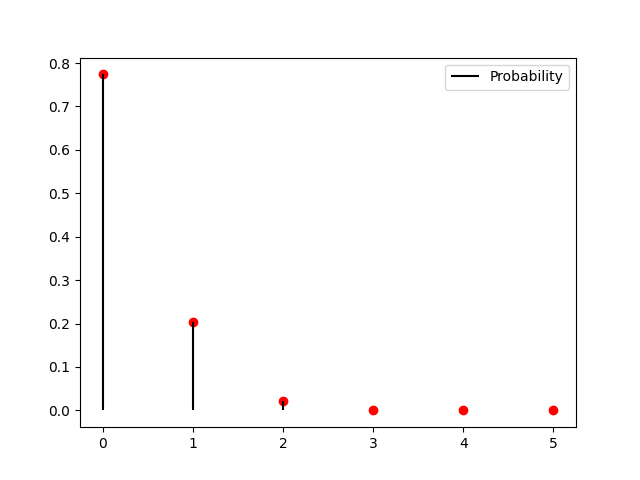
\includegraphics[width=\textwidth,height=5.5cm,keepaspectratio]{figures/PMF.png}
		\caption{Probability Mass Function}
		\label{fig1}
	\end{figure}
\end{frame}

\begin{frame}{CDF Graph}
The CDF graph is:
    \begin{figure}[!ht]
		\centering
		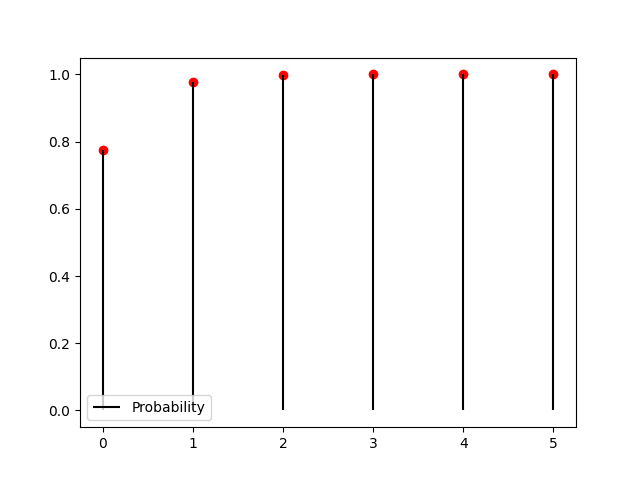
\includegraphics[width=\textwidth,height=5.5cm,keepaspectratio]{figures/CDF.png}
		\caption{Cumulative Distribution Function}
		\label{fig2}
	\end{figure}
\end{frame}


\end{document}